\documentclass[xcolor={x11names,svgnames}, 14pt]{beamer}
\setbeamerfont{note page}{size=\tiny} % default = small 


%\includeonlyframes{applications}


\usecolortheme{rose}
\setbeamertemplate{footline}{}
\setbeamertemplate{navigation symbols}{\footnotesize\insertframenumber}
  
\usepackage{amsmath, amssymb, amsthm}

\usepackage[utf8]{inputenc}
\usepackage[francais]{babel}
\usepackage[T1]{fontenc}
\usepackage[normalem]{ulem}   
\usepackage{mdframed}
\usepackage{multirow}

\usepackage{minted}
%\setminted{fontsize=\scriptsize}

\usepackage{tikz}
\usetikzlibrary{calc}
\usetikzlibrary{decorations}
\usetikzlibrary{positioning}
\usetikzlibrary{decorations.pathmorphing}
\usetikzlibrary{decorations.pathreplacing}
\usetikzlibrary{shapes.multipart}
\usetikzlibrary{math}

\usepackage{fontspec}

\setsansfont{PalatinoSansLTPro}[
   Path = /home/charles/charles_work/fonts/PalatinoSans/, 
   Extension      = .otf,
   UprightFont    = *-Regular,
   BoldFont= *-Bold ,
   ItalicFont = *-Italic,
   BoldItalicFont = *-BoldIta
]

\newcommand{\blue}[1]{{\color{Blue}#1}}
%\newcommand{\green}[1]{{\color{LimeGreen}#1}}
\newcommand{\red}[1]{{\color{red}#1}}
\newcommand{\tikzmat}[2] {
\draw[thick] let \p1 = (#1 |- #2),
                 \p2 = (#2 |- #1) in
   ($ (#1) + (0.05,-0.1) $) -- ++(-0.15, 0)  -- ($ (\p1) + (-0.1,0.1) $) -- ++(0.15,0)
   ($ (\p2) + (-0.05,-0.1) $) -- ++(0.15, 0) -- ($ (#2) + (0.1,0.1) $) -- ++(-0.15,0);
}


\author[C.~Bouillaguet]{Charles Bouillaguet \newline
  {\small \texttt{charles.bouillaguet@univ-lille.fr}}}

\title{Cours 9 : puissance de crête, équilibrage, intensité opérationnelle, etc.}
%\date{2020-02-28}




\begin{document}

\begin{frame}[label=title]
    \titlepage
  \end{frame}
  
%%%%%%%%%%%%%%%%%

\begin{frame}
  \frametitle{Jeu de rôle}
  \framesubtitle{Vous êtes le CNRS et vous venez de vous faire livrer}
  \centering
  \begin{columns}
    \begin{column}{4.75cm}
      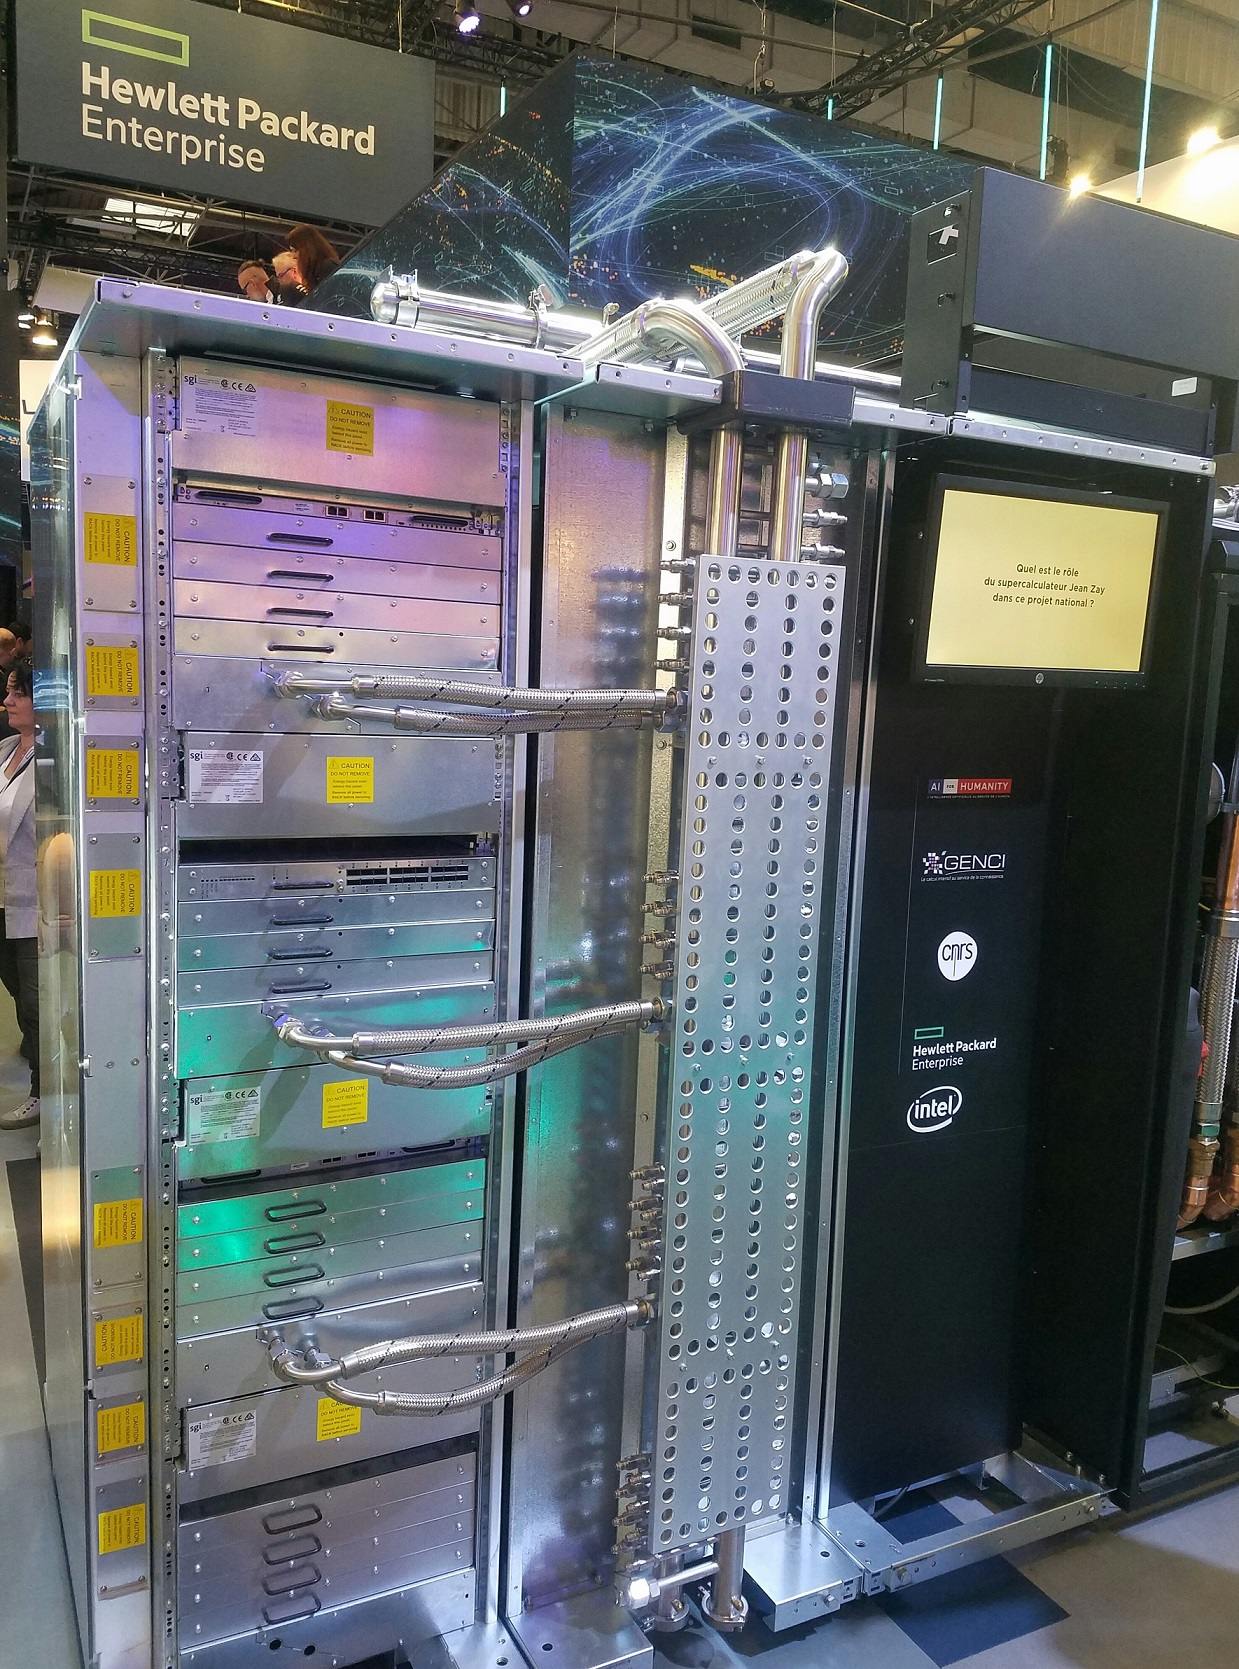
\includegraphics[height=7cm]{jean-zay}
    \end{column}
    \begin{column}{5.5cm}
      \small
      \begin{itemize}
      \item 1528 noeuds
      \item 2 $\times$ Xeon Gold 6248 (\og Cascade Lake\fg{})
      \item 20 coeurs @ 2.5 Ghz
      \item 192 Go RAM/noeud
      \item Omnipath 100Gbit/s
      \end{itemize}

      \begin{block}{Question légitime}
        À quel point ça va aller plus vite que le précédent ?
      \end{block}
    \end{column}
  \end{columns}
\end{frame}

%%%%%%%%%%%%%%%%%%%

\begin{frame}
  \frametitle{Puissance de crête}

  \begin{block}{Définition}
    Nombre maximal de FLOPS que le hardware peut (en théorie) effectuer.
  \end{block}

  \begin{itemize}
  \item Noeuds
  \item SMP ?
  \item Fréquence CPU
  \item Coeurs
  \item Unités SIMD
  \item Parallélisme d'instruction
  \item Fused Multiply-Add
  \end{itemize}
  
\end{frame}

%%%%%%%%%%%%%%%%

\begin{frame}
  \frametitle{Cas facile}
  \framesubtitle{Turing}

  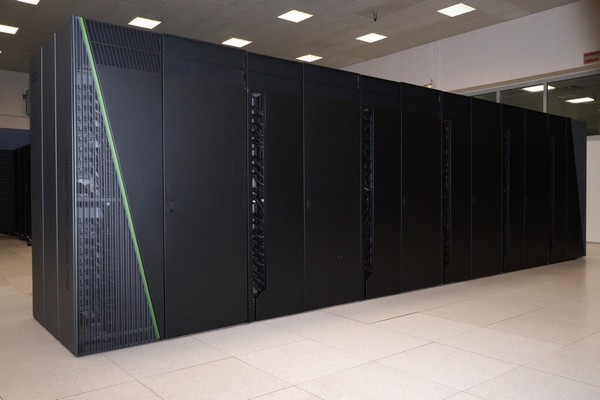
\includegraphics[width=\textwidth]{turing}
\end{frame}

\begin{frame}
  \frametitle{Cas facile}
  \framesubtitle{Turing}

  \begin{itemize}
  \item Noeuds : 6144
  \item CPU : PowerPC A2 @ 1.6Ghz
  \item Coeurs : 16
  \item Unités SIMD : 256-bits (4 doubles)
  \item Fused Multiply-Add : oui
  \item 1 instruction/cycle maximum
  \end{itemize}

  \begin{alertblock}{Résultat}
    $6144 \times 1.6e9 \times 16 \times 4 \times 2 = 1144$ TeraFLOPS
  \end{alertblock}
\end{frame}

%%%%%%%%%%%%%%%%%%%

\begin{frame}
  \frametitle{Cas dur}
  \framesubtitle{Jean-Zay}

  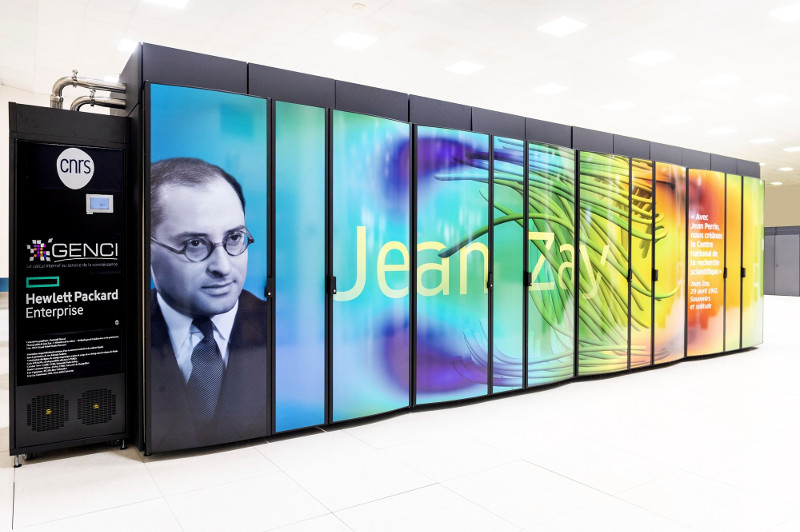
\includegraphics[width=\textwidth]{jean-zay-bis}
\end{frame}

\begin{frame}
  \frametitle{Cas dur}
  \framesubtitle{Jean-Zay}

  \begin{itemize}
  \item Noeuds : 1528
  \item CPU Xéon Gold 6248 @ \alert{[ça dépend]} GHz
  \item Coeurs : 20
  \item Unités SIMD : 512-bits (8 doubles)
  \item Fused Multiply-Add : oui
  \item instruction/cycle maximum : \alert{2 FMA}
    \begin{itemize}
    \item Xeon Bronze \& Silver : 1 seul.
    \item Xeon Gold \& Platinum : 2.
    \end{itemize}
  \end{itemize}
\end{frame}

%%%%%%%%%%%%%%%%

\begin{frame}
  \frametitle{CPU Frequency Scaling}
  \framesubtitle{Problème d'enveloppe thermique}
  
  \begin{block}{La fréquence d'un coeur dépend}
  \begin{itemize}
  \item Du type d'instruction exécuté
  \item De ce que font les autres coeurs
  \item De la qualité du composant matériel
  \end{itemize}
\end{block}

\bigskip

\centering
  \small
\begin{tabular}{|c|c||c|c|c|c|c|c|c|c|}
  \hline
  \multirow{2}{*}{Mode}   & \multirow{2}{*}{Base} & \multicolumn{6}{c|}{Turbo avec $x$ coeurs actifs} \\
%  \cline{3-23}
  & &             1-2 & 3-4 & 5-8 & 9-12 & 13-16 & 17-20 \\
  \hline\hline
  normal & 2.5	& 3.9 & 3.7 & 3.6 & 3.6 & 3.4 & 3.2 \\
  \hline
  AVX2	 & 1.9	& 3.8 & 3.6 & 3.5 & 3.4 & 3.0 & 2.8 \\
  \hline
  AVX512 & 1.6	& 3.8 & 3.6 & 3.5 & 3.0 & 2.7 & 2.5 \\
  \hline
\end{tabular}
\end{frame}

%%%%%%%%%%%%

\begin{frame}
  \frametitle{Intensité Opérationnelle}

  \begin{block}{Rappel}
    On cherche à prévoir/comprendre les performances d'une application sur une machine donnée.
  \end{block}

  \begin{exampleblock}{Définition}
    L'\alert{intensité opérationnelle} d'un algorithme est le nombre
    d'opérations arithmétiques effectuées par octet transféré depuis la RAM.
  \end{exampleblock}
  
  \[
    IO = \dfrac{\text{FLOP}}{\text{Octets }\leftrightarrow\text{ RAM}}
  \]
\end{frame}

%%%%%%%%%%%%%%%%%%%%%%%%%

\begin{frame}
  \frametitle{Intensité Opérationnelle}
  \framesubtitle{Intérêt}
  
    \centering
    \scalebox{0.8}{
      $\text{[FLOPS]} \leq \max \bigl( [\text{peak FLOPS}],  [IO] \times [\text{peak RAM BW}]\bigr)$
    }

  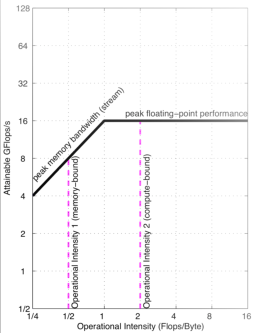
\includegraphics[height=6cm]{roofline_basic.pdf}
\end{frame}

%%%%%%%%%%%%%%%%%%%%%%%%% 

\begin{frame}[fragile]
  \frametitle{Intensité Opérationnelle}
  \framesubtitle{Petits exemples}
  
  \begin{block}{Produit scalaire}
\begin{minted}{C}
double res = 0;
for (int j = 0; j < N; j++)
    res += A[i] * B[i];
\end{minted}
  \end{block}

  \pause

  \bigskip

  \[
    IO = 1/8.
  \]  
\end{frame}

%%%%%%%%%%%%%%%%%%%%%%%%%

\begin{frame}[fragile]
  \frametitle{Intensité Opérationnelle}
  \framesubtitle{Petits exemples}
  
  \begin{block}{Produit matrice-vecteur}
\begin{minted}{C}
for (int i = 0; i < N; i++) {
    y[i] = 0.0;
    for (int j = 0; j < N; j++)
        y[i] += A[i*N + j] * x[j];
}
\end{minted}
  \end{block}

  \pause

  \bigskip

  \[
    IO = \begin{cases}
      1 / 4 & \text{ si $x$ tient en cache} \\
      1 / 8 & \text{ sinon}
    \end{cases}
  \]  
\end{frame}

%%%%%%%%%%%%%%%%%%%%%%%%%

\begin{frame}[fragile]
  \frametitle{Intensité Opérationnelle}
  \framesubtitle{Petits exemples}
  
  \begin{block}{Produit matrice creuse-vecteur dense}
\begin{minted}{C}
for (int i = 0; i < n; i++) {
  y[i] = 0;
  for (int u = Ap[i]; u < Ap[i+1]; u++) {
    int j = Aj[u];
    y[i] += Ax[u] * x[j];
  }
}
\end{minted}
  \end{block}

  \pause

  \[
    IO = \begin{cases}
      1 / 6  & \text{ si $x$ tient en cache} \\
      1 / 10 & \text{ sinon}
    \end{cases}
  \]  
\end{frame}

%%%%%%%%%%%%%%%%%%%%%%%%%

\begin{frame}[fragile]
  \frametitle{Améliorer l'intensité opérationnelle ?}

  \begin{itemize}
  \item En général, il faut changer les algos...
  \item Optimisation generique : \emph{loop fusion}.
  \end{itemize}

  \bigskip
  
  \begin{columns}
    \begin{column}{0.5\textwidth}
\begin{minted}[fontsize=\scriptsize]{C}
/* Mauvais */
for (int i = 0; i < N; i++)
    A[i] = B[i] * C[i];
for (int i = 0; i < N; i++)
    D[i] = B[i] + E[i];
\end{minted}
    \end{column}
    \begin{column}{0.5\textwidth}
\begin{minted}[fontsize=\scriptsize]{C}
/* Meilleur */
for (int i = 0; i < N; i++) {
    A[i] += B[i] * C[i];
    D[i] += B[i] + E[i];
}
\end{minted}
    \end{column}
  \end{columns}
\end{frame}

%%%%%%%%%%%%%%%%%%%%%

\begin{frame}[fragile]
  \frametitle{Application : dans le projet...}

\begin{minted}[fontsize=\small]{C}
for (int i = 0; i < n; i++) {
   x[i] += alpha * p[i];
   r[i] -= alpha * q[i];
   z[i] = r[i] / d[i];
}
rz = dot(n, r, z);
\end{minted}

  \medskip
  \hrule
  \medskip

\begin{minted}[fontsize=\small]{C}
rz = 0
for (int i = 0; i < n; i++) {
   x[i] += alpha * p[i];
   r[i] -= alpha * q[i];
   z[i] = r[i] / d[i];  // on pouvait l'éliminer...
   rz += r[i] * z[i];
}
\end{minted}

\end{frame}

%%%%%%%%%%%%%%%%%%%%%%%%%%

\begin{frame}
  \frametitle{Retour sur le projet}

  \begin{alertblock}{Dans la plupart des cas...}
    \begin{itemize}      
    \item Temps de calcul dominé par SPMV
      \begin{itemize}
      \item Matrice creuse $\times$ vecteur dense
      \end{itemize}
    \item Matrice grosse (e.g. Serena = 800 Mo)
    \item Vecteur petit (n $\approx 10^6$, 8Mo $\rightarrow$ OK cache L3)
    \item[$\Rightarrow$] Intensité arithmétique $\approx 1/6$.
    \end{itemize}
  \end{alertblock}
\end{frame}

%%%%%%%%%%%%%%%%%%%%%%%%%%%

\begin{frame}
  \frametitle{Diagramme \og Roofline\fg{}}
  \centering
  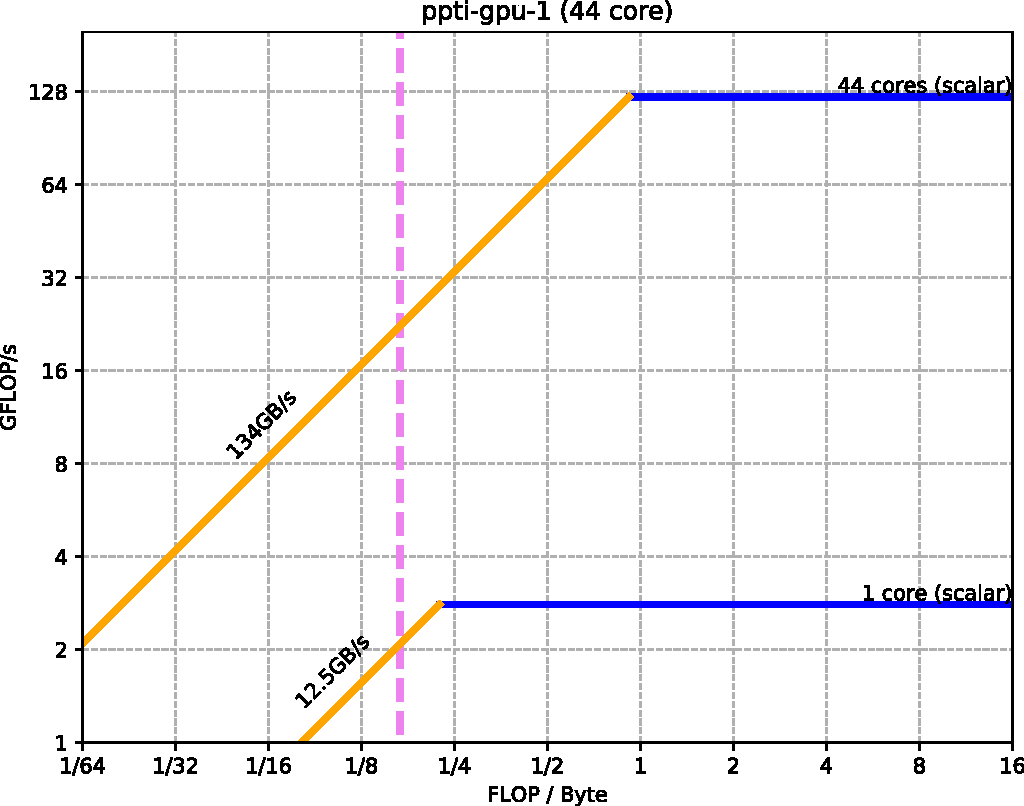
\includegraphics[width=\textwidth]{roofline_ppti.pdf}
\end{frame}


%%%%%%%%%%%%%%%%%%%%%%%%%%%

\begin{frame}
  \frametitle{Diagramme \og Roofline\fg{}}
  \centering
  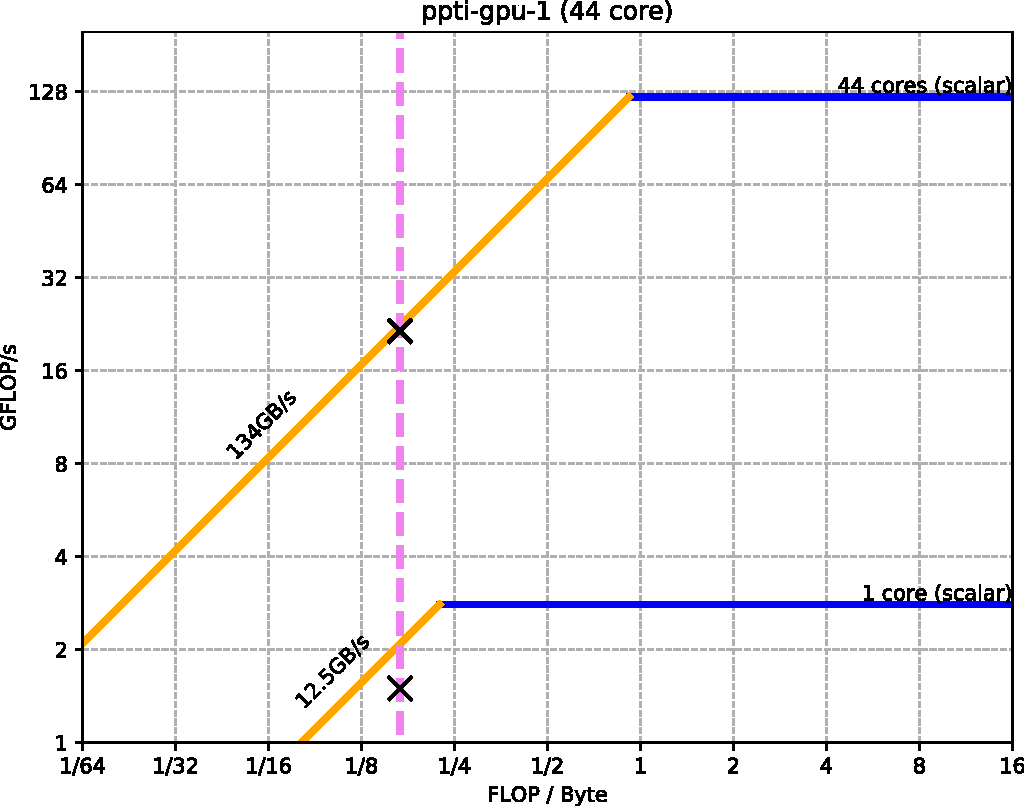
\includegraphics[width=\textwidth]{roofline_ppti2.pdf}
\end{frame}

%%%%%%%%%%%%%%%%%%%%%%%%%%%%%%

\begin{frame}
  \frametitle{On peut aussi le faire avec le réseau !}

  \begin{block}{Solution naïve}
    \begin{itemize}
    \item Vecteurs réparti entre $p$ noeuds.
    \item On a besoin de tout $x$ pour faire $y \gets A\cdot x$...
    \item[$\Rightarrow$] \texttt{MPI\_Allgather} à chaque itération sur $x$
    \item Chaque noeud reçoit $8n \frac{p-1}{p}$ octets / itération.
    \item Une itération $\approx 2W$ FLOP (dans SPMV)
    \end{itemize}
  \end{block}

  \begin{alertblock}{Dans la PPTI}
    Gigabit ethernet = 128Mo/s \small (dans le meilleur des cas)
  \end{alertblock}

  \only<1>{$8n \times [\text{itération/s}] \leq 128 \cdot 10^6$}
  \only<2>{$8n \times [\text{FLOPS}] / 2W \leq 128 \cdot 10^6$}
  \only<3>{$[\text{FLOPS}] \leq 32 \frac{W}{n} \cdot 10^6 $}
  
\end{frame}

%%%%%%%%%%%%%%%%%%%%%%%%%%%%%

\begin{frame}
  \frametitle{On peut aussi le faire avec le réseau !}
  
  \begin{block}{Matrice \og Serena\fg{}}
    \begin{itemize}
    \item $n = 1.4e6$ et $W = 64e6$
    \item 2 GigaFLOPS et 14 itération/s sur un poste.
    \end{itemize}
  \end{block}

  \begin{overlayarea}{\textwidth}{5cm}
  \begin{alertblock}<only@1>{Si on passe par le réseau de la PPTI...}
    \begin{itemize}
    \item $[\text{FLOPS}] \leq 32 \frac{W}{n} \cdot 10^6 $
    \item[$\Rightarrow$] $\leq 1.6$ GigaFLOPS (à cause du réseau)
    \end{itemize}
  \end{alertblock}

  \begin{exampleblock}<only@2>{Si on avait un \textbf{meilleur} réseau ?}
    \begin{itemize}
    \item Infiniband/Omnipath à 100 Gigabit/s ?
    \item $[\text{FLOPS}] \leq 32 \frac{W}{n} \cdot 10^{\alert{8}}$
    \item[$\Rightarrow$] $\leq 163$ GigaFLOPS (à cause du réseau)
    \item[$\Rightarrow$] $82$ noeuds ont assez de FLOPS pour saturer
    \end{itemize}
  \end{exampleblock}
\end{overlayarea}
\end{frame}


%%%%%%%%%%%%%%%%%%%%%%%%%%%%%%

\begin{frame}
  \frametitle{Modèle I/O simplifié}

  \begin{block}{Hypothèses}
  \begin{itemize}
  \item Mémoire \textbf{lente} (grosse ; e.g. RAM).
  \item Mémoire \textbf{rapide} (petite ; e.g. cache).
  \item CPU relié à la mémoire rapide uniquement.
  \item Transferts CPU $\leftrightarrow$ rapide = \alert{gratuit}.
  \end{itemize}
\end{block}

\begin{itemize}
  \item $\nu$ FLOP, $\mu$ doubles transférés ($IO = \frac{\nu}{8\mu}$). 
  \item Un FLOP : $t_\nu$. Un transfert : $t_\mu$.
  \end{itemize}
%  \vspace{-0.25cm}
  \[
  T = \nu \times t_\nu \pause + \mu \times t_\mu \pause = \nu \times t_\nu \left(1 + \frac{t_\mu}{t_\nu} \times \only<3>{\frac{\mu}{\nu}}\only<4>{\frac{1}{8IO}} \right)
\]

\end{frame}

%%%%%%%%%%%%%%%%%%%%%%%%%%%

% Serena
% % # equations:   1,391,349                                           
% # non-zeroes: 64,531,701                                           

% sequential
%     ---> CSR matrix size = 796.6Mbyte
%     ---> Working set : 846.7Mbyte
% ---> Per iteration: 1.3e+08 FLOP in sp_gemv() and 1.7e+07 FLOP in the rest
% ---> error : 8.29e+00, iter : 215 (10.0 it/s, 1.46 GFLOPs)^C
%     ---> Finished in 129.1s and 1344 iterations

% stream : 12 Go/s (1 thread)
% stream : max BW = 134Go/s (88 threads)

% 88 threads :
% ---> Finished in 8.9s and 1328 iterations

%spmv
	% for (int i = 0; i < n; i++) {
	% 	y[i] = 0;
	% 	for (int u = Ap[i]; u < Ap[i + 1]; u++) {
	% 		int j = Aj[u];
	% 		double A_ij = Ax[u];
	% 		y[i] += A_ij * x[j];
	% 	}
        %       }
        %       W * 20 bytes + 2W FLOP

        %           for (int i = 0; i < n; i++) {
        %                 x[i] += alpha * p[i];
        %                 r[i] -= alpha * q[i];
        %                 z[i] = r[i] / d[i];
        %           }
        %           rz = dot(n, r, z);
        %           double beta = rz / old_rz;
        %           for (int i = 0; i < n; i++)
        %             p[i] = z[i] + beta * p[i];
        %   7n double + 9n flops
              
              

\end{document}





%%% Local Variables:
%%% TeX-command-extra-options: "-shell-escape"
%%% TeX-engine: xetex
%%% ispell-local-dictionary: "french"
%%% eval: (flyspell-mode 1)
%%% eval: (reftex-mode 1)
%%% End:
